\documentclass[dvipdfmx]{jsarticle}
\usepackage{tikz}
\begin{document}

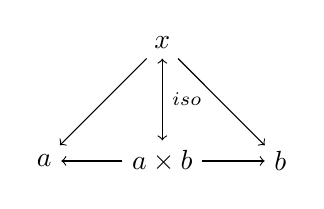
\begin{tikzpicture}[auto]
  \node (ab) at (1.5, 0) {$a\times b$};
  \node (a) at (0, 0) {$a$};
  \node (b) at (3, 0) {$b$};

  \node (x) at (1.5, 1.5) {$x$};
  \draw[<->] (x) to node {$\scriptstyle iso$} (ab);

  \draw[->] (ab) to node {} (a);
  \draw[->] (ab) to node {} (b);
  \draw[->] (x) to node {} (a);
  \draw[->] (x) to node {} (b);



\end{tikzpicture}



\begin{tikzpicture}[auto]
  \node (aone) at (1.5, 0) {$a\times 1$};
  \node (a) at (0, 0) {$a$};
  \node (one) at (3, 0) {$1$};

  \node (aa) at (1.5, 1.5) {$a$};
  \draw[<->] (aa) to node {$\scriptstyle iso$} (aone);

  \draw[->] (aone) to node {} (a);
  \draw[->] (aone) to node {} (b);
  \draw[->] (aa) to node[swap] {$\scriptstyle id_a$} (a);
  \draw[->] (aa) to node {$\scriptstyle !_a$} (one);
  \end{tikzpicture}

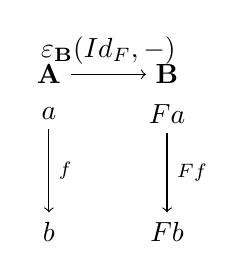
\begin{tikzpicture}[auto]
  \node (catA) at (1.5, 2) {$\mathbf{A}$};
  \node (catB) at (3, 2) {$\mathbf{B}$};
  \draw[->] (catA) to node {$\varepsilon _\mathbf{B}(Id_F,-)$} (catB);

  \node (a) at (1.5, 1.5) {$a$};
  \node (b) at (1.5, 0) {$b$};

  \node (Fa) at (3, 1.5) {$Fa$};
  \node (Fb) at (3, 0) {$Fb$};

  \draw[->] (a) to node {$\scriptstyle f$} (b);
  \draw[->] (Fa) to node {$\scriptstyle Ff$} (Fb);

  \end{tikzpicture}
\end{document}
